\section{Monidas Plattform}
\label{mon}
Die Monidas-Plattform bildet die technische Grundlage für den Monidas Code Aist Navigator. In diesem Kapitel wird die bestehende Monidas-Plattform beschrieben, um die Ausgangslage für die entwickelte Lösung besser zu verstehen.

\subsection{Plattform}
Die Monidas-Plattform ist eine von der Colomba Link GmbH entwickelte IoT-Plattform, die auf die Überwachung von Sensordaten spezialisiert ist. Sie dient als zentrale Lösung zur Erfassung, Verarbeitung und Darstellung von Echtzeitdaten aus vernetzten Geräten. Ziel der Plattform ist es, Unternehmen bei der effizienten Überwachung und Optimierung ihrer komplexen Infrastrukturen und Prozesse zu unterstützen. Die erfassten Sensordaten werden auf der Monidas-Plattform in einer Benutzeroberfläche dargestellt, wie in Abbildung \ref{fig:mon_plat} gezeigt. Dabei werden aktuelle Messwerte sowie zeitliche Entwicklungen (z. B. Verlauf der Temperatur und Luftfeuchtigkeit) angezeigt, sodass Nutzer Veränderungen schnell erkennen und die Daten einfach interpretieren können.

\begin{figure}[H]
  \centering
  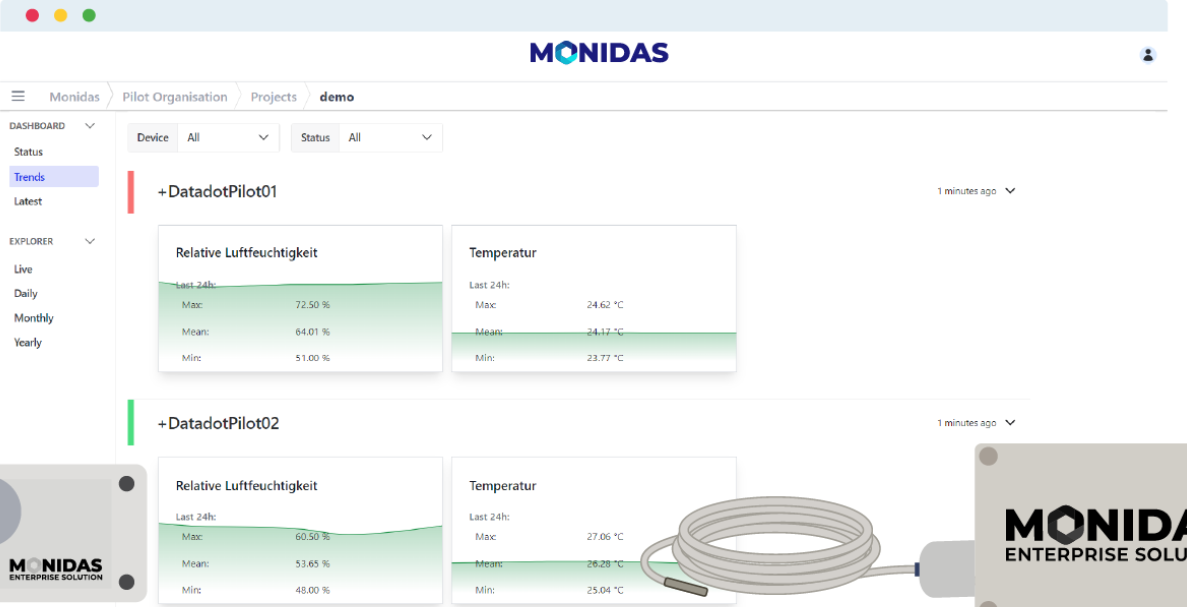
\includegraphics[width=1\linewidth]{mon_plat.png}
  \caption{}
  \label{fig:mon_plat}
\end{figure}

Die in Abbildung \ref{fig:mon_plat} dargestellte Übersicht setzt voraus, dass zuvor mehrere Entitäten der Monidas-Plattform eingerichtet und miteinander verknüpft wurden. Der hierfür notwendige Konfigurationsprozess wurde bereits in Kapitel \ref{kap:konf} beschrieben und bildet nur einen Teil der gesamten Funktionalität der Plattform ab. Im Folgenden werden nun gezielt jene Entitäten vorgestellt, deren Verständnis für die Umsetzung und Evaluation des Monidas Code Assist Navigators besonders relevant ist. Aufgrund der Komplexität und des Umfangs des vollständigen Domänenmodells beschränkt sich die Darstellung bewusst auf einen relevanten Ausschnitt, welcher anschliessend anhand eines vereinfachten UML-Diagramms in Abbildung \ref{fig:mon_UML} veranschaulicht wird.
\newpage

\begin{}\begin{itemize}
  \item \textbf{Organization}: Organisationen.
  \item \textbf{Project}: Projekte, die einer Organisation zugeordnet sind.
  \item \textbf{User}: Personen, die einer Organisation oder einem Projekt zugeordnet sind.
  \item \textbf{Function}: Wertet Sensordaten aus und ermittelt daraus den Zustand des Sensors.
  \item \textbf{Template}: Vorlage, welche den Betreff und Inhalt von Benachrichtigungen definiert.
  \item \textbf{Group}: Vorlage, die festlegt, welche Personen Benachrichtigungen erhalten.
  \item \textbf{Action}: Benachrichtigt definierte Empfänger bei bestimmten Sensorereignissen.
  \item \textbf{Device}: Physische Geräte (z. B. Sensoren), die Daten erfassen und übertragen.
  \item \textbf{Monitor}: Überwachungseinheiten, die Sensordaten überwachen und eine Action auslösen.
\end{itemize}


\begin{figure}[H]
  \centering
  \includegraphics[width=1\linewidth]{mon_UML.png}
  \caption{}
  \label{fig:mon_UML}
\end{figure}


\subsection{Technologien}